%%%%%%%%%%%%%%%%%%%%%%%%%%%%%%%%%%%%%%%%%
% baposter Landscape Poster
% LaTeX Template
% Version 1.0 (11/06/13)
%
% baposter Class Created by:
% Brian Amberg (baposter@brian-amberg.de)
%
% This template has been downloaded from:
% http://www.LaTeXTemplates.com
%
% License:
% CC BY-NC-SA 3.0 (http://creativecommons.org/licenses/by-nc-sa/3.0/)
%
%%%%%%%%%%%%%%%%%%%%%%%%%%%%%%%%%%%%%%%%%

%----------------------------------------------------------------------------------------
%	PACKAGES AND OTHER DOCUMENT CONFIGURATIONS
%----------------------------------------------------------------------------------------

\documentclass[landscape,a0paper,fontscale=0.3]{baposter} % Adjust the font scale/size here

\usepackage{float} % Required for multiple columns
\usepackage{placeins}
\usepackage{stfloats}
\usepackage[utf8]{inputenc}
\usepackage[T1]{fontenc}
\usepackage[french]{babel}

\usepackage{graphicx} % Required for including images
\graphicspath{{figures/}} % Directory in which figures are stored

\usepackage{amsmath} % For typesetting math
\usepackage{amssymb} % Adds new symbols to be used in math mode

\usepackage{booktabs} % Top and bottom rules for tables
\usepackage{enumitem} % Used to reduce itemize/enumerate spacing
\usepackage{palatino} % Use the Palatino font
\usepackage[font=small,labelfont=bf]{caption} % Required for specifying captions to tables and figures

\usepackage{multicol} % Required for multiple columns
\setlength{\columnsep}{1.5em} % Slightly increase the space between columns
\setlength{\columnseprule}{0mm} % No horizontal rule between columns
\selectcolormodel{cmyk}

\usepackage{tikz} % Required for flow chart
\usetikzlibrary{shapes,arrows} % Tikz libraries required for the flow chart in the template

\newcommand{\compresslist}{ % Define a command to reduce spacing within itemize/enumerate environments, this is used right after \begin{itemize} or \begin{enumerate}
\setlength{\itemsep}{1pt}
\setlength{\parskip}{0pt}
\setlength{\parsep}{0pt}
}

\definecolor{darkgreen}{cmyk}{0.2394,0.0000,0.2394,0.2627}
\definecolor{orange}{cmyk}{0.0000,0.7294,1.0000,0.0000} 
\definecolor{floralwhite}{cmyk}{0.0000,0.0196,0.0588,0.0000}
\definecolor{gray}{cmyk}{0.0000,0.0000,0.0000,0.0392}
\definecolor{lightgreen}{cmyk}{0.7554,0.0000,0.7554,0.4549}
\definecolor{lightblue}{rgb}{0.145,0.6666,1} % Defines the color used for content box headers

\begin{document}

\begin{poster}
{
headerborder=closed, % Adds a border around the header of content boxes
colspacing=1em, % Column spacing
bgColorOne=floralwhite, % Background color for the gradient on the left side of the poster
bgColorTwo=white, % Background color for the gradient on the right side of the poster
borderColor=lightgreen, % Border color
headerColorOne=lightgreen, % Background color for the header in the content boxes (left side)
headerColorTwo=white, % Background color for the header in the content boxes (right side)
headerFontColor=white, % Text color for the header text in the content boxes
boxColorOne=white, % Background color of the content boxes
textborder=roundedleft, % Format of the border around content boxes, can be: none, bars, coils, triangles, rectangle, rounded, roundedsmall, roundedright or faded
eyecatcher=true, % Set to false for ignoring the left logo in the title and move the title left
headerheight=0.1\textheight, % Height of the header
headershape=roundedright, % Specify the rounded corner in the content box headers, can be: rectangle, small-rounded, roundedright, roundedleft or rounded
headerfont=\large\bf\textsc, % Large, bold and sans serif font in the headers of content boxes
%textfont={\setlength{\parindent}{1.5em}}, % Uncomment for paragraph indentation
linewidth=2pt % Width of the border lines around content boxes
}
%----------------------------------------------------------------------------------------
%	TITLE SECTION 
%----------------------------------------------------------------------------------------
%
{
\includegraphics[height=6em]{logo_lip_HD}} % First university/lab logo on the left
{\bf\Large\textcolor{orange}{Caractérisation et Méthodologie d'Analyse des Buffer Overflow }\vspace{0.2em}} % Poster title
{\textsl{ \small Yves KONE, Stella BITCHEBE, Alain TCHANA \{Ecole Normale Supérieure de Lyon\}\\ \vspace{0.2em}

\includegraphics[width=0.2\linewidth]{compas18}}} % Author names and institution
{
\includegraphics[height=6em]{enslogo}} % Second university/lab logo on the right

%----------------------------------------------------------------------------------------
%	OBJECTIVES
%----------------------------------------------------------------------------------------

\headerbox{CVE: Common Vulnerabilities and Exposures}{name=cve,column=0,row=0,span=2}{
\small{
% Le buffer overflow est la vulnérabilité la plus répandue \cite{top25} Les CVE pour Common Vuln\'erabilites and Exposures est une base de donn\'ees publique r\'epertoriant des vuln\'erabili\'es de s\'ecurité.
L'ensemble des vulnérabilités de sécurité est répertorié dans une base de données publique sous le nom de CVE.
Les CVE constituent un jeu de donn\'ees important pour la recherche en s\'ecurité\cite{dowser}.
Chaque entrée dans la base de données est composée de 2 parties disctinctes:
\begin{itemize}
	\item Le descriptif principal qui pr\'esente bri\`evement la vuln\'erabilité
    \item Les r\'ef\'erences qui sont des URLs vers des pages web de diff\'erents types
\end{itemize}
\begin{center}
    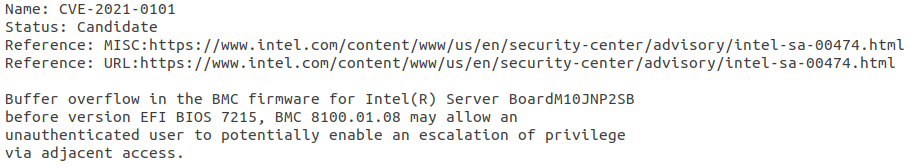
\includegraphics[width=0.7\linewidth, height=2.1cm]{cve_entry}
    \captionof{figure}{Extrait du CVE de type buffer overflow (ou BOF) 2021-2182.}
    \end{center}}
%\vspace{0.1em} % When there are two boxes, some whitespace may need to be added if the one on the right has more content
}

\headerbox{Challenge}{name=challenge,column=1, below=cve, span=1}{
\small{Le principal challenge est de d\'eterminer les caract\'eristiques d'un buffer overflow.
En effet les informations \'etant non structur\'ees il est assez compliqué de \textcolor{red}{XXX}:
\begin{itemize}
    \item \bf Le type de d\'ebordement
    \item \bf La zone m\'emoire
    \item \bf Les cons\'equences ou effets
    \item \bf Le contexte relatif au code
    \item \bf Le syst\`eme impacté
    \item \bf La compagnie, entreprise impact\'ee
\end{itemize}
}
}
%----------------------------------------------------------------------------------------
%	RESULTS 
%----------------------------------------------------------------------------------------



%----------------------------------------------------------------------------------------
%	REFERENCES
%----------------------------------------------------------------------------------------



%----------------------------------------------------------------------------------------
%	CONTACT INFORMATION
%----------------------------------------------------------------------------------------


%----------------------------------------------------------------------------------------
%	CONTRIB
%----------------------------------------------------------------------------------------



%----------------------------------------------------------------------------------------
%	PROBLEM
%----------------------------------------------------------------------------------------





\headerbox{Problématique}{name=problem,column=0,below=cve, bottomaligned=challenge}{ % This block's bottom aligns with the bottom of the conclusion block
\small{Les buffers overflow consitituent la vulnérabilité la plus répandue \cite{top25}.
Neanmoins, une analyse \textbf{fine et pertinente} des CVE pour les extraire peut s'av\'erer une tâche tr\`es \textbf{longue et fastidieuse}.\newline
Les principales causes sont:}
\begin{itemize}
    \item \bf\textcolor{orange}{Le grand nombre de CVE r\'epertorié (12669 CVE concernant les overflow depuis 2013)}
	\item \bf\textcolor{orange}{Les donn\'ees sont non structur\'ees} 
    \item \bf\textcolor{orange}{Aucune m\'ethode d'analyse connue ou d'outil automatique, il faut tout \'etudier soit-m\^eme \`a la main}
\end{itemize}
}

\headerbox{Résultats Préliminaires}{name=results,column=2,span=2,row=0}{
Les figures~\ref{fig:1}-\ref{fig:4} présentent quelques résutlats obtenus après une analyse rigoureuse de \textbf{368 CVEs} de type \textbf{buffer overflow} pour l'année 2021.
\begin{multicols*}{2}
    \begin{figure}[H]
        \vspace{0.6cm}
        \centering
        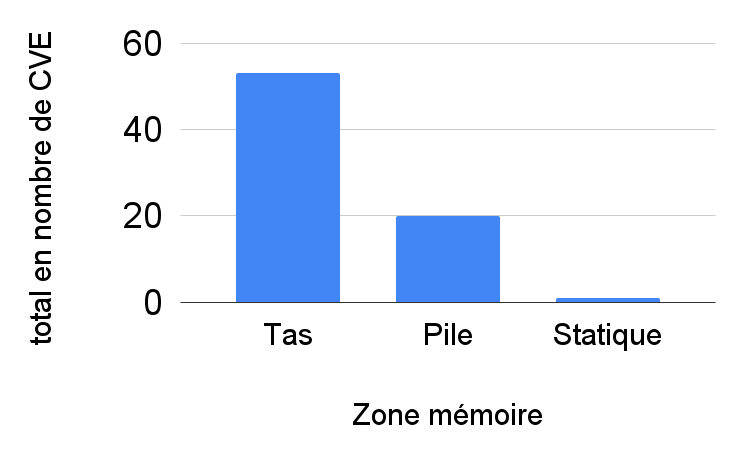
\includegraphics[width=0.7\linewidth, height=3.6cm]{zone}
        \captionof{figure}{Nombre de CVE par type de zone concernée.}
        \label{fig:1}
    \end{figure}
    \begin{figure}[H]
        \centering
        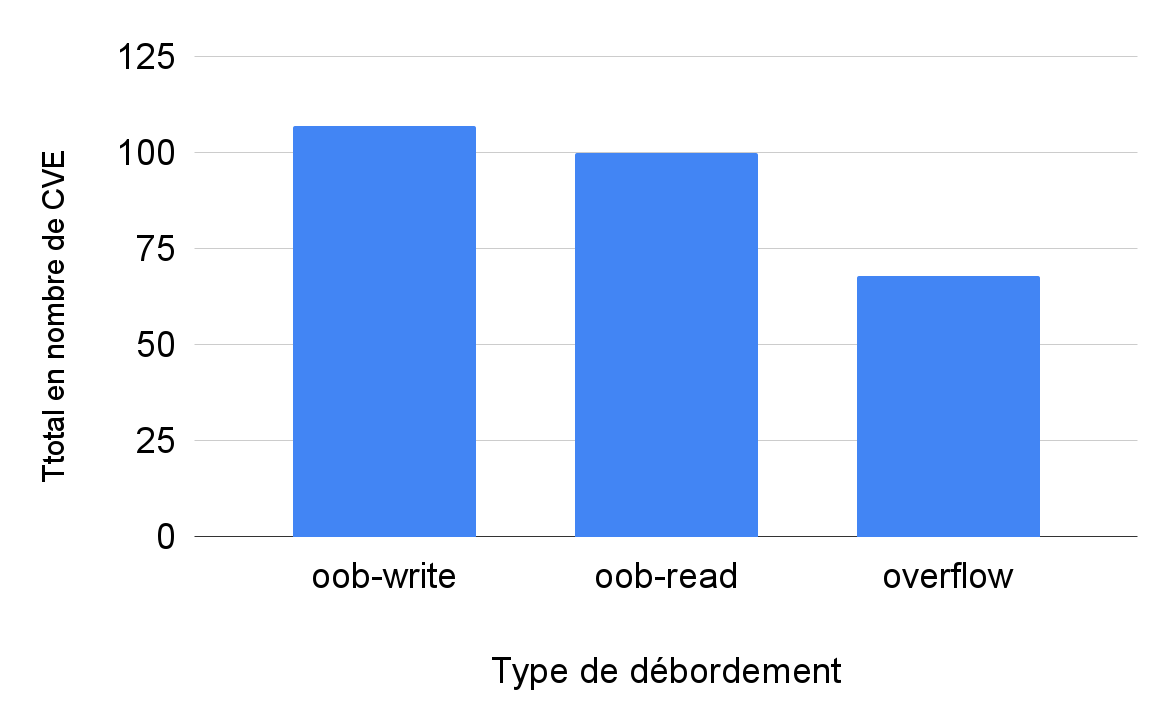
\includegraphics[width=0.9\linewidth, height=4.2cm]{debordement.png}
        \captionof{figure}{Nombre de CVE par type de d\'ebordement.}
        \label{fig:2}
    \end{figure}
    \begin{figure}[H]
        \centering
        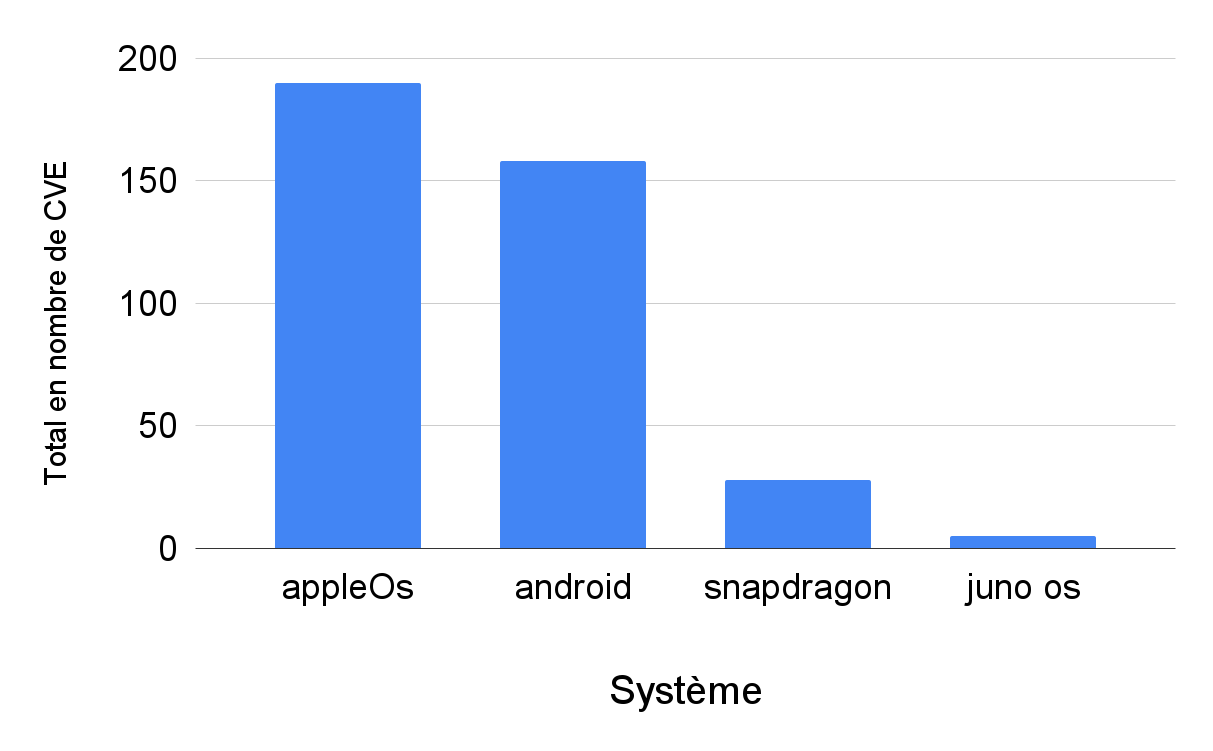
\includegraphics[width=0.9\linewidth, height=4.2cm]{systeme}
        \captionof{figure}{Nombre de CVE par syst\`eme impacté.}
        \label{fig:3}
    \end{figure}
    \begin{figure}[H]
        \centering
        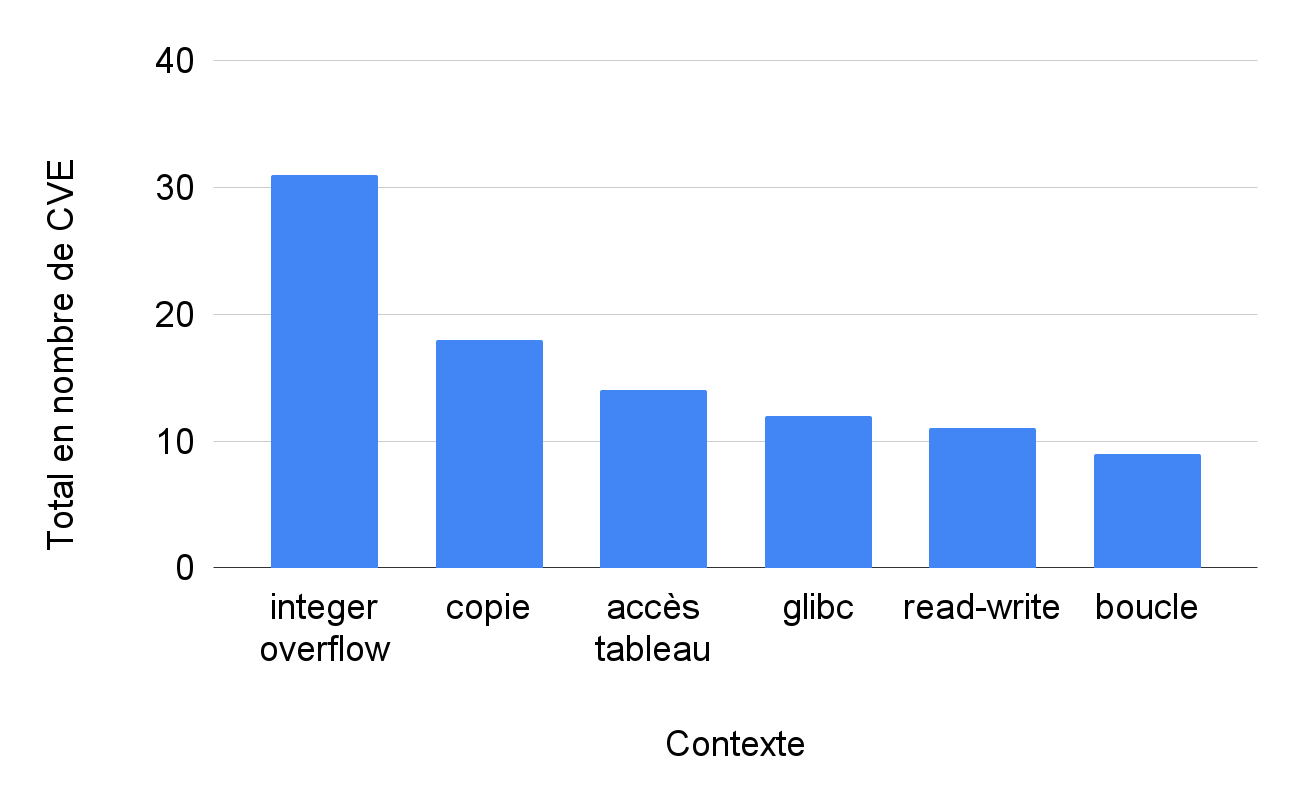
\includegraphics[width=0.9\linewidth, height=4.2cm]{contexte}
        \captionof{figure}{Nombre de CVE par syst\`eme impacté.}
        \label{fig:4}
    \end{figure}
\end{multicols*}
}
%----------------------------------------------------------------------------------------
%	MOTIV
%----------------------------------------------------------------------------------------

%----------------------------------------------------------------------------------------



\headerbox{Contact}{name=contact,column=2, span=2,above=bottom,boxColorOne=floralwhite}{ % This block is as tall as the references block
\begin{multicols}{2}
    
\begin{description}\compresslist
\item[Email] yves.kone@ens-lyon.fr
\item[Email] celestine-stella.ndonga-bitchebe@ens-lyon.fr
\vspace{2cm}
\item[Email] alain.tchana@ens-lyon.fr
\end{description}
\end{multicols}

}



\headerbox{Méthodologie}{name=contrib,below=problem, above=bottom,column=0,span=2,row=0}{
L'algorithme d'extraction de CVE est divisé en 2 parties: l'\'etude du descriptif principal puis de chacune des r\'ef\'erences.
Pour l'étude du descriptif, qui est constitué de texte brut en langage humain, il faut simplement \textbf{\emph{extraire}} les informations relatives à la caract\'erisation d\'efinie et les \textbf{interpréter} correctement.
\begin{figure}[H]
    \centering
    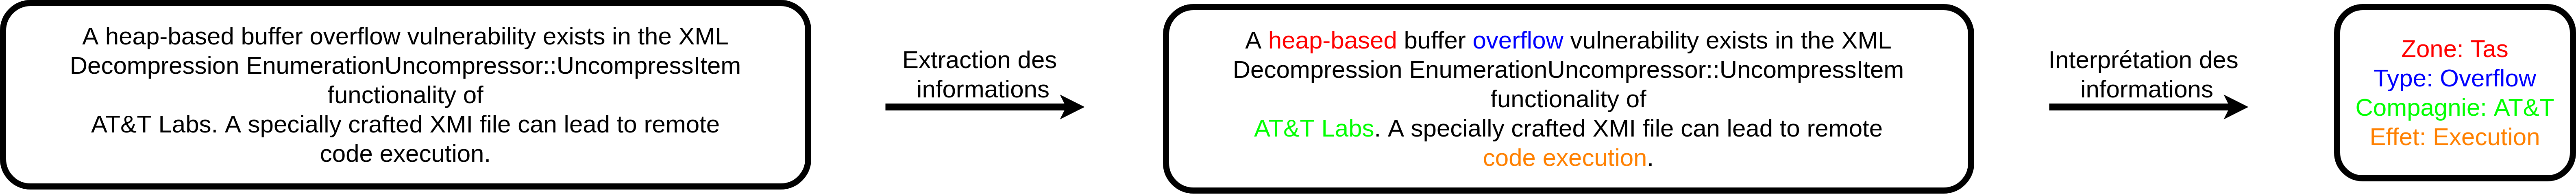
\includegraphics[width=16.5cm, height=1.3cm]{descriptif}
    \captionof{figure}{Extrait du descriptif du cve 2021-2182.}
\end{figure}
\vspace{-0,2cm}

Pour les références, il faut tout d'abord \textbf{identifier} le type de page web \textcolor{red}{ça veut dire quoi??} dont il s'agit et ensuite les sources d'information dans la page web. Ces sources sont en général constituées de texte et peuvent être de nature différentes (titre, code, etc...).
Enfin, comme pour le descriptif \textbf{extraire} les donn\'ees et les \textbf{interpr\'eter}.
    \begin{figure}[H]
        \centering
        
\includegraphics[width=16cm, height=2.3cm]{reference}
        \captionof{figure}{Automate simplifié de l'analyse des r\'ef\'erences d'un cve. \textcolor{red}{-->> elle est hors du cadre!!}}
    \end{figure}
}


\headerbox{Travaux Futurs}{name=comments, span=2,column=2,below=results}{La conception d'un outil pour :
%\vspace{0.4cm}
\begin{itemize}
    \item \bf\textcolor{orange}{Extraire et interpr\'eter du texte correctement malgré avec un tol\'erance aux fautes;}
    \item \bf\textcolor{orange}{Identifier, pour chaque type de page web, les sources d'informations potentielles et en extraire les donn\'ees clefs;}
    \item \bf\textcolor{orange}{Généraliser la méthode pour d'autres types de vulnérabilités.}
\end{itemize}
}


\headerbox{Références}{name=references,column=2,above=contact,span=2,below=comments,boxColorOne=floralwhite}{

\renewcommand{\section}[2]{\vskip 0.05em} % Get rid of the default "References" section title
\nocite{*} % Insert publications even if they are not cited in the poster
\small{ % Reduce the font size in this block
\bibliographystyle{unsrt}
\bibliography{sample} % Use sample.bib as the bibliography file
}}
\end{poster}

\end{document}